\chapter{Introduction}
\label{chapter: introduction}
% * motivate why robots should operate in a human world 
In 1961 the first industrial robot Unitmate was put to work \cite{noauthor_unimate_2022}. From that point on, industrial robots proved very successful in factories. At the assembly line, robots do predefined tasks in a known environment. Research and engineering expanded and improved the robot's abilities over the years. In recent decades a new ability has gained attention, operating in other environments than at the factory floor. Such as in people's homes, in supermarkets or in a hospital. These environments are changing fast and contain a variety of objects, making them more complex and more unpredictable. As a result the robot operates in a environment which is less defined compared to the factory floor. To operate in these lesser defined environments robots need to be more autonomous compared to the assembly line counterpart. There do not yet exist mature solutions to the arisen challenges which autonomous robots need to overcome, explaining why creating autonomous robots which can operate in unpredictable fast-changing environments is such a hot research topic nowadays. Although autonomous robots are a hot topic in research, it has gained less attention from the industry. Companies such as \href{https://www.bostondynamics.com/}{Boston Dynamics} or \href{http://www.siasun.com/index.php?m=content&c=index&a=initsa}{SIASUN} 
create autonomous robots that are promising with potential, but there is still a lot to improve before autonomous robots can be called a success. \\

% * Motivate why having knowledge of the environment increases task performance
One challenge of a autonomous robot is to define the environment with the objects in it. To motivate why the robot should need knowledge of the environment it operates in, a comparison with ourselves is made. For us humans, mostly we are rewarded if we improve our interactions, such as typing is faster with 10 fingers instead of 2 which makes you type faster, or improving playing an instrument gives the joy of being able to play more interesting music. Learning is thus rewarded. Which nature understood  because nature fine-tuned humans to understand the world we live in. Already in the womb, a baby learns that it can move, that is has arms. A small child always seems to grasp everything, in a lot of cases to check if it is edible. Children go through a phase where they question almost everything to understand the world around them. Because if you understand the world around you, it's easier to accomplish tasks. For example, a barista who works at a coffee bar can struggle with just a few customers on the first day, but after a month he/she can provide coffee for large groups effortless because of an increased understanding of coffee and the coffee bar. \\

For autonomous robots, finding a action sequence to fulfil a task is hard, because actions taken now influence the future state of the environment, successful completion bears uncertainty and actions cannot always be rolled back. In this literature study, improving robots to be more autonomous is investigated in 2 areas. The \textbf{first} one is having system models of objects to describe their dynamics. A robot can interact with objects by grasping, pushing, pulling or manipulate objects in other ways (e.g. throwing, kicking). Different objects react differently to, for example a push by the robot. How these objects react can be captured with system models. The true system dynamics are dominated by nonlinear dynamics, contains uncertain parameters and can change over time, which is why autonomous robots need to constantly monitor. It is assumed that if the model estimation improves, manipulation improves. \textbf{Secondly}, to have more autonomous robots, attention should be paid to task planning because of the influence of current action on future tasks. In this report we investigate the most prominent task planning techniques such as backward induction \cite{krontiris_dealing_2015}. The scope of this literature is formalised through the following problem description.\\
% describe the problem such that it is clear
% it is about learning dynamical properties of objects, what objects are. 
% Task an motion planning in a unknown environment
% A task is defined

\section{Research Question}
\label{section: research_question}
The main question is separated into multiple subquestions.\\

\textbf{Main research question:}
\begin{center}
\large
    Can objects' system models be learned by a robot during task execution, and can these newly learned models improve task,  motion and manipulation planning?
\end{center} 

\textbf{Research subquestion:}
\begin{enumerate}
    \item \label{researchsubquestion: system_models} How are system models learned, and what are the limitations for different system learning techniques.
    \item\label{researchsubquestion: piecewise_analytic} Why is task, motion and manipulation planning so much more difficult compared to task and motion planning.
    \item \label{researchsubquestion: proposed_method} Can planning in configuration space be extended to a piece-wise analytic configuration space with learned dynamics. 
\end{enumerate}
\section{Problem Description}
\label{section: problem_description}
In this literature we focus on the problem of task, motion, and manipulation planning in a simplified simulated environment where a robot is commanded to push possibly unknown object to target locations. This is a well investigated problem in the literature \cite{sabbagh_novin_model_2021,wang_affordance-based_2020,scholz_navigation_2016,siciliano_path_2009, goldberg_asymptotically_2020} and it touches on both system identification and task planning.\\
    
Assumption \ref{assumption: closed_world}, \ref{assumption: quasi_static}, \ref{assumption: perfect_object_sensor}, \ref{assumption: order_does_not_matter} and \cref{definition: robot_world} fully define the environment. \\

\begin{assumption}
\label{assumption: closed_world}
\textbf{Closed-World Assumption:} Objects are manipulated, directly or indirectly only by the robot. Objects cannot be manipulated by influences from outside the environment.
\end{assumption}

\begin{assumption}
\label{assumption: quasi_static}
\textbf{Quasi-Static Assumption:} Velocities are small enough that inertial forces are negligible \cite{stuber_lets_2020}, thus objects only move if manipulated by the robot.
\end{assumption}

\begin{assumption}
\label{assumption: perfect_object_sensor}
\textbf{Perfect Object Sensor Assumption:} the robot has full access to the poses and geometry of all objects in the environment at all times.
\end{assumption}

\begin{assumption}
\label{assumption: order_does_not_matter}
\textbf{Task are Commutative} Tasks exist of multiple objects with specified target positions. The order in which objects are pushed toward their target position is commutative.
\end{assumption}

\begin{definition}
\label{definition: robot_world} \textbf{Environment description}\\
The robot environment consists of a flat ground plane, gravity pulls all 3-dimensional objects perpendicular toward the ground plane. Let tuple $<g, Origin, Ob, E>$ define the world, where:
\begin{itemize}
    \item $g$ is the gravity constant.
    \item $Origin$ is the worlds origin from where the position and orientation can be defined.
    \item $Ob$ is a set of be a set of objects $ob_1, ob_2, \dots, ob_n$.
    \item $E$ is a set of motion equations which describe the behaviour of objects and interaction between objects. The motion equations coincide with the true dynamics, in a simulation environment these are known, in the real world the motion equations are unknown.
\end{itemize} 

Each object contains mass, a center of gravity, geometry and a state consisting of position, velocity, orientation and angular velocity $< pos_x, pos_y, pos_z, pos_\theta, pos_\gamma, pos_\rho, vel_x, vel_y, vel_z, vel_\theta, vel_\gamma, vel_\rho>$. The state of an object $i$ is expressed in short hand notation state $s_i$ of an object $ob_i$.  
\end{definition}

% motivate multiple controllers
Now the robot's environment has been defined, let's look at the robot. The robot is a mobile robot, without any grippers. The only action which is can take is driving around, structure about the robot's driving dynamics is assumed to be known because the robot can be analysed during design and construction. Details about the robot remain unknown such as the exact radius of the robot's wheels, and mass because such parameters can change over time, system identification could estimate such parameters. Interaction with object can be performed by bumping into objects to perform a push. The robot contains a set of controllers and various methods to identify the objects system model. Because controllers use different types of models the term 'system model' generalises all models which capture the real dynamics and are able to simulate future states of objects as a function of the current states and robot inputs. The combination of a controller and a compatible system model can be used to navigate the robot in the environment. \\

% describe what a task is
A configuration $c_i$ associated with object $ob_i$ is defined as a subset of the object's state $c_i \subseteq s_i$. A task is defined as set of desired configuration of objects, containing one or more objects with associated configurations. Such a desired set of configurations, or target configurations do have some rules to adhere to. It is required that every object can at most have one target configuration, and objects cannot be overlapping with other objects target configuration, including geometry of the object. Task must be commutative, see assumption \ref{assumption: order_does_not_matter}. The target configuration must be stable (so no object floating above the ground or orientations such that is tips over). The robot  is commanded by means of driving and pushing to put the objects from their current state in their target configuration with an certain threshold. Above mentioned requirements do not make every task feasible, the robot could be trapped by unmovable objects, or the target is to move an object to heavy to push.\\

A robot having knowledge about the environment's objects and true dynamics is expected to be more efficient in reaching the target configurations compared to a robot without any knowledge. This literature investigates this claim providing a number of related works and their analysis. \\

% Intro of the environment
\begin{figure}[H]
    \centering
    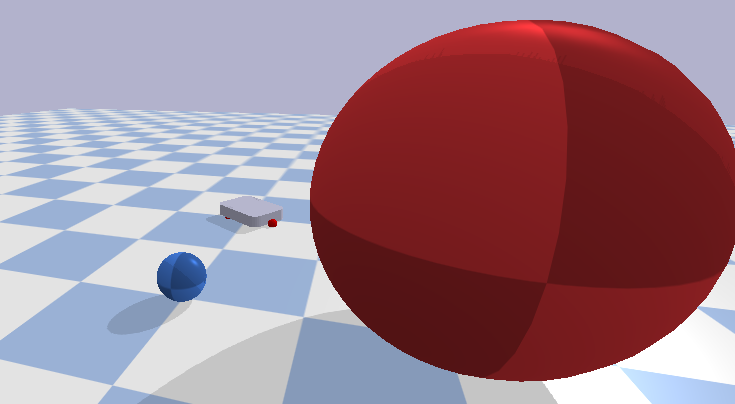
\includegraphics[width=0.6\textwidth]{figures/example_robot_world.png}
    \caption{An example world with the boxer robot and 2 sphere obstacles}
    \label{figure: example_world_intro}
\end{figure}

In a more practical setup, a simulation is used to create the robot environment. \Cref{figure: example_world_intro} is an example of such an environment. Before running the simulation, the robot is provided with the geometry of every object, objects do not change geometry during simulation. When simulating the environment the robot is updated with objects states for every time step. What is unknown it the objects' weights and the set of motion equations $E$. 

\section{Report Structure}
\label{section: report_structure}
So far, an introduction, problem description and research questions has been presented. The goal was to narrow down the problem at hand, give a clear overview of the robot environment. \\

\Cref{chapter: interaction_with_env_and_model_identification} answers the first research subquestion. Before an answer can be given, system models are categorised in  \cref{section: system_model_representation}, followed by a categorisation of control methods that can make use of the system models in \cref{section: interaction_approaches_and_model_iden_methods}. The first research subquestion is then answered in \cref{section: controllers_discussion}.\\

\Cref{chapter: task_and_motion_planning} gives an overview of \ac{TAMP} methods, split in a section for motion and manipulation planning in \cref{section: toward_target_pose}, and a section for task planning in \cref{section: toward_sequence_target_poses}.
Research subquestion \cref{researchsubquestion: piecewise_analytic} is then answered in the discussion \cref{section: tamp_discussion}.\\

\Cref{chapter: proposed_method} drafts a new method to overcome the limitations shown in \cref{chapter: interaction_with_env_and_model_identification} and \cref{chapter: task_and_motion_planning}. This new method introduces the \textit{hypothesis graph} in \cref{section: hgraph} and introduces the \textit{knowledge graph} in  
\cref{section: knowledge_graph}. \Cref{section: btests} creates a variety of environments with tasks for the robot to fulfil. These test display the expected hypothesis graph and expected knowledge graph indicating how the proposed method completes tasks. Finally the last research subquestion is answered in \cref{section: proposed_method_discussion}. \\

\Cref{chapter: conclusion} will provide a brief summary of the discussion sections followed by an answer to the main research question. 

